\documentclass[12pt]{article}
\renewcommand{\labelenumii}{\theenumii}
\renewcommand{\theenumii}{\theenumi.\arabic{enumii}.}

\usepackage[utf8]{inputenc}
\usepackage[margin=1.0in]{geometry}
\usepackage{amsmath}
\usepackage{amssymb}
\usepackage{graphicx}
\graphicspath{ {C:/Users/james/workspace/ds5/written/images/} }

\title{Homework 5 Written (36 points)}
\author{James Shin (js4785)}
\date{Due: April 28, 2016}


\begin{document}
\maketitle

\section{Exercise 9.1}
Topological sort gives us the following table. The numbers in the chart denote indegrees before dequeue, the top row indicates the vertex number in the topological sort, and the bottom two rows indicate the order in which vertices are enqueued and dequeued.
\begin{center}
\begin{tabular}{ c|c|c|c|c|c|c|c|c|c|c|c } 
vertex & 1 & 2 & 3 & 4 & 5 & 6 & 7 & 8 & 9 & 10 & 11 \\
 \hline
 $s$ & 0 & 0 & 0 & 0 & 0 & 0 & 0 & 0 & 0 & 0 & 0 \\
 A & 2 & 1 & 1 & 0 & 0 & 0 & 0 & 0 & 0 & 0 & 0 \\
 B & 1 & 1 & 1 & 1 & 1 & 0 & 0 & 0 & 0 & 0 & 0 \\
 C & 3 & 3 & 3 & 3 & 3 & 3 & 2 & 1 & 1 & 0 & 0 \\
 D & 2 & 1 & 0 & 0 & 0 & 0 & 0 & 0 & 0 & 0 & 0 \\
 E & 4 & 4 & 3 & 2 & 1 & 0 & 0 & 0 & 0 & 0 & 0 \\
 F & 2 & 2 & 2 & 2 & 2 & 2 & 2 & 1 & 1 & 0 & 0 \\
 G & 1 & 0 & 0 & 0 & 0 & 0 & 0 & 0 & 0 & 0 & 0 \\
 H & 1 & 1 & 0 & 0 & 0 & 0 & 0 & 0 & 0 & 0 & 0 \\
 I & 2 & 2 & 2 & 2 & 1 & 1 & 1 & 0 & 0 & 0 & 0 \\
 $t$ & 3 & 3 & 3 & 3 & 3 & 3 & 3 & 3 & 2 & 1 & 0 \\
 \hline
 enqueue & $s$ & G & D,H & A &  & B,E &  & I & F & C & $t$ \\
 dequeue & $s$ & G & D & H & A & B & E & I & F & C & $t$ \\
\end{tabular}
\end{center}

So the final topological ordering is $\boxed{s,G,D,H,A,B,E,I,F,C,t}$

\section{Exercise 9.7a}
\begin{center}
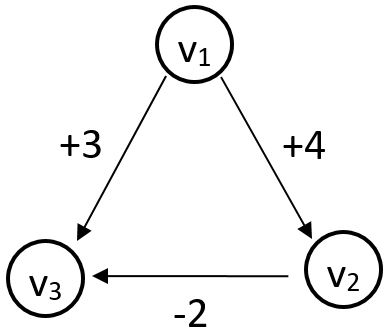
\includegraphics[scale=0.5]{97pic1}
\end{center}
The graph above gives the wrong answer in the presence of a negative edge but no negative-cost cycle. Running Dijkstra's algorithm, we get:
\begin{center}
\begin{tabular}{ c c c c } 
vertex & known & $d_v$ & $p_v$ \\
 \hline
$v_1$ & F & 0 & 0 \\
$v_2$ & F & $\infty$ & 0 \\
$v_3$ & F & $\infty$ & 0 \\
\end{tabular}
$\rightarrow$
\begin{tabular}{ c c c c } 
vertex & known & $d_v$ & $p_v$ \\
 \hline
$v_1$ & T & 0 & 0 \\
$v_2$ & F & 4 & $v_1$ \\
$v_3$ & F & 3 & $v_1$ \\
\end{tabular}
$\rightarrow$
\begin{tabular}{ c c c c } 
vertex & known & $d_v$ & $p_v$ \\
 \hline
$v_1$ & T & 0 & 0 \\
$v_2$ & F & 4 & $v_1$ \\
$v_3$ & T & 3 & $v_1$ \\
\end{tabular}
$\rightarrow$
\begin{tabular}{ c c c c } 
vertex & known & $d_v$ & $p_v$ \\
 \hline
$v_1$ & T & 0 & 0 \\
$v_2$ & T & 4 & $v_1$ \\
$v_3$ & T & 3 & $v_1$ \\
\end{tabular}
\end{center}

We see that the $d_v$ for $v_3$ is not correct, since the shortest is actually $2$ if the path from $v_1$ to $v_2$ to $v_3$ is considered.

\section{Question 9.15}
First we perform Prim's Algorithm:
\begin{center}
\begin{tabular}{ c c c c } 
vertex & known & $d_v$ & $p_v$ \\
 \hline
$A$ & F & 0 & 0 \\
$B$ & F & $\infty$ & 0 \\
$C$ & F & $\infty$ & 0 \\
$D$ & F & $\infty$ & 0 \\
$E$ & F & $\infty$ & 0 \\
$F$ & F & $\infty$ & 0 \\
$G$ & F & $\infty$ & 0 \\
$H$ & F & $\infty$ & 0 \\
$I$ & F & $\infty$ & 0 \\
$J$ & F & $\infty$ & 0 \\
\end{tabular}
$\rightarrow$
\begin{tabular}{ c c c c } 
vertex & known & $d_v$ & $p_v$ \\
 \hline
$A$ & T & 0 & 0 \\
$B$ & F & 3 & A \\
$C$ & F & $\infty$ & 0 \\
$D$ & F & 4 & A \\
$E$ & F & 4 & A \\
$F$ & F & $\infty$ & 0 \\
$G$ & F & $\infty$ & 0 \\
$H$ & F & $\infty$ & 0 \\
$I$ & F & $\infty$ & 0 \\
$J$ & F & $\infty$ & 0 \\
\end{tabular}
$\rightarrow$
\begin{tabular}{ c c c c } 
vertex & known & $d_v$ & $p_v$ \\
 \hline
$A$ & T & 0 & 0 \\
$B$ & T & 3 & A \\
$C$ & F & 10 & B \\
$D$ & F & 4 & A \\
$E$ & F & 2 & B \\
$F$ & F & 3 & B \\
$G$ & F & $\infty$ & 0 \\
$H$ & F & $\infty$ & 0 \\
$I$ & F & $\infty$ & 0 \\
$J$ & F & $\infty$ & 0 \\
\end{tabular}
$\rightarrow$
\begin{tabular}{ c c c c } 
vertex & known & $d_v$ & $p_v$ \\
 \hline
$A$ & T & 0 & 0 \\
$B$ & T & 3 & A \\
$C$ & F & 10 & B \\
$D$ & F & 4 & A \\
$E$ & T & 2 & B \\
$F$ & F & 3 & B \\
$G$ & F & $\infty$ & 0 \\
$H$ & F & 2 & E \\
$I$ & F & 1 & E \\
$J$ & F & $\infty$ & 0 \\
\end{tabular}
$\rightarrow$
\begin{tabular}{ c c c c } 
vertex & known & $d_v$ & $p_v$ \\
 \hline
$A$ & T & 0 & 0 \\
$B$ & T & 3 & A \\
$C$ & F & 10 & B \\
$D$ & F & 4 & A \\
$E$ & T & 2 & B \\
$F$ & F & 3 & B \\
$G$ & F & $\infty$ & 0 \\
$H$ & F & 2 & E \\
$I$ & T & 1 & E \\
$J$ & F & 7 & I \\
\end{tabular}
$\rightarrow$
\begin{tabular}{ c c c c } 
vertex & known & $d_v$ & $p_v$ \\
 \hline
$A$ & T & 0 & 0 \\
$B$ & T & 3 & A \\
$C$ & F & 10 & B \\
$D$ & F & 4 & A \\
$E$ & T & 2 & B \\
$F$ & F & 3 & B \\
$G$ & F & $\infty$ & 0 \\
$H$ & T & 2 & E \\
$I$ & T & 1 & E \\
$J$ & F & 7 & I \\
\end{tabular}
$\rightarrow$
\begin{tabular}{ c c c c } 
vertex & known & $d_v$ & $p_v$ \\
 \hline
$A$ & T & 0 & 0 \\
$B$ & T & 3 & A \\
$C$ & F & 6 & F \\
$D$ & F & 4 & A \\
$E$ & T & 2 & B \\
$F$ & T & 3 & B \\
$G$ & F & 2 & F \\
$H$ & T & 2 & E \\
$I$ & T & 1 & E \\
$J$ & F & 7 & I \\
\end{tabular}
$\rightarrow$
\begin{tabular}{ c c c c } 
vertex & known & $d_v$ & $p_v$ \\
 \hline
$A$ & T & 0 & 0 \\
$B$ & T & 3 & A \\
$C$ & F & 1 & G \\
$D$ & F & 4 & A \\
$E$ & T & 2 & B \\
$F$ & T & 3 & B \\
$G$ & T & 2 & F \\
$H$ & T & 2 & E \\
$I$ & T & 1 & E \\
$J$ & F & 7 & I \\
\end{tabular}
$\rightarrow$
\begin{tabular}{ c c c c } 
vertex & known & $d_v$ & $p_v$ \\
 \hline
$A$ & T & 0 & 0 \\
$B$ & T & 3 & A \\
$C$ & T & 1 & G \\
$D$ & F & 4 & A \\
$E$ & T & 2 & B \\
$F$ & T & 3 & B \\
$G$ & T & 2 & F \\
$H$ & T & 2 & E \\
$I$ & T & 1 & E \\
$J$ & F & 7 & I \\
\end{tabular}
$\rightarrow$
\begin{tabular}{ c c c c } 
vertex & known & $d_v$ & $p_v$ \\
 \hline
$A$ & T & 0 & 0 \\
$B$ & T & 3 & A \\
$C$ & T & 1 & G \\
$D$ & T & 4 & A \\
$E$ & T & 2 & B \\
$F$ & T & 3 & B \\
$G$ & T & 2 & F \\
$H$ & T & 2 & E \\
$I$ & T & 1 & E \\
$J$ & F & 7 & I \\
\end{tabular}
$\rightarrow$
\begin{tabular}{ c c c c } 
vertex & known & $d_v$ & $p_v$ \\
 \hline
$A$ & T & 0 & 0 \\
$B$ & T & 3 & A \\
$C$ & T & 1 & G \\
$D$ & T & 4 & A \\
$E$ & T & 2 & B \\
$F$ & T & 3 & B \\
$G$ & T & 2 & F \\
$H$ & T & 2 & E \\
$I$ & T & 1 & E \\
$J$ & T & 7 & I \\
\end{tabular}

\end{center}

\newpage

Now we perform Kruskal's Algorithm.
\begin{center}
\begin{tabular}{ c c c } 
Edge & Weight & action \\
 \hline
$(C,G)$ & 1 & Accepted \\
$(E,I)$ & 1 & Accepted \\
$(B,E)$ & 2 & Accepted \\
$(E,H)$ & 2 & Accepted \\
$(F,G)$ & 2 & Accepted \\
$(A,B)$ & 3 & Accepted \\
$(B,F)$ & 3 & Accepted \\
$(F,I)$ & 3 & Rejected \\
$(A,D)$ & 4 & Accepted \\
$(A,E)$ & 4 & Rejected \\
$(H,I)$ & 4 & Rejected \\
$(D,E)$ & 5 & Rejected \\
$(C,F)$ & 6 & Rejected \\
$(D,H)$ & 6 & Rejected \\
$(I,J)$ & 7 & Accepted \\
\end{tabular}
\end{center}
The graph below shows the resulting minimum spanning tree using either Prim's or Kruskal's Algorithm.
\begin{center}
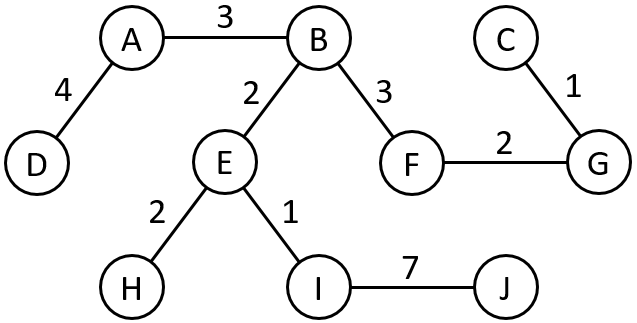
\includegraphics[scale=0.6]{915pic1}
\end{center}

\section{Question 9.20}
To find the maximum spanning tree, we can simply just negate all the edge weights on the graph and perform the exact same algorithm as the minimum spanning tree algorithm (either Prim's or Kruskal's) to find the maximum spanning tree. Once finished, change the edge weights back to its original values. Note this works since the minimum spanning tree algorithm accounts for negative edge weights.

\newpage

\section{Question 9.21}
We build the following depth-first spanning tree, starting at vertex $A$. We see that $Low(B) \geq Num(C)$, $Low(H) \geq Num(E)$, and $Low(G) \geq Num(F)$, which means that $C$, $E$, and $F$ are all articulation points in the graph. This is verifiable; deleting any of these three articulation points in the original graph causes the graph to become disconnected.
\begin{center}
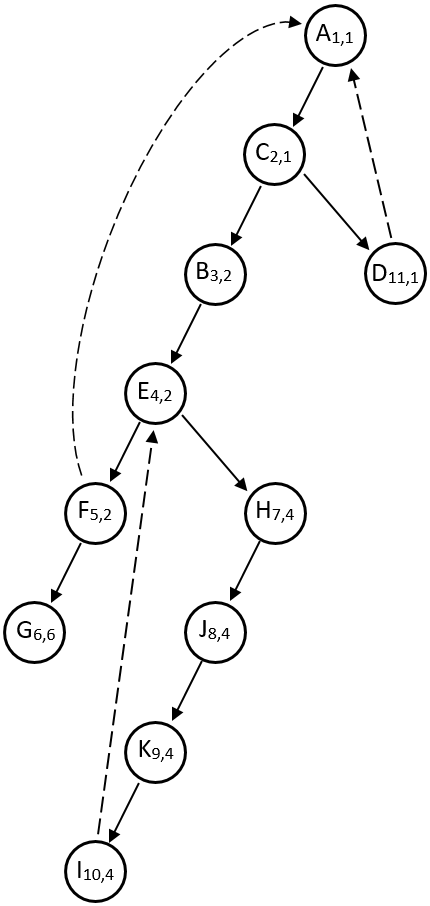
\includegraphics[scale=0.8]{921pic1}
\end{center}

\newpage

\section{Question 9.38}
\renewcommand{\theenumi}{\alph{enumi}}
\begin{enumerate}
\item For two sticks $a$ and $b$, look at the $x$ and $y$ coordinates of their endpoints. Write a linear equation for each pair of endpoints for the two sticks and check to see whether the two intersect in between the bounds of their endpoints; in other words, check to see whether the line segments made by the $x$ and $y$ coordinates of the two sticks intersect. If they do intersect, then compare their $z$ coordinates to see which stick is on top of which. If they do not interect, then the two sticks $a$ and $b$ are not related.
\item We will utilize a topological sorting algorithm. Each stick is represented by a vertex on a directed graph. If you can remove some stick $v$ before some other stick $w$, $i.e.$ $v$ is on top of some stick $w$, then put a directed edge from $v$ to $w$. Then performing topological sort will give a valid pick-up ordering that you can perform in order to pick up all the sticks. If there is a cycle in the topological sort, that means that all of the sticks cannot be picked up, and therefore there would exist no valid sequence of stick pickups.
\end{enumerate}

\end{document}